%% LONG VERSION (first draft, 17 November 2026, 43 pages). Superseded by ../main.tex; kept as the source of the supplement.
%% Every number in the text is produced by a script in validation/ (see NOTES.md).
%% Lines starting with "%% TODO" are open points for the authors.
\documentclass[preprint,12pt]{elsarticle}

\usepackage{amssymb}
\usepackage{amsmath}
\usepackage{amsthm}
\usepackage{siunitx}
\usepackage{booktabs}
\usepackage{graphicx}
\usepackage[hidelinks]{hyperref}
\renewcommand{\figureautorefname}{Figure}
\renewcommand{\tableautorefname}{Table}
\renewcommand{\sectionautorefname}{Section}
\renewcommand{\subsectionautorefname}{Section}
\usepackage[all]{hypcap}

\graphicspath{{../../validation/}}

%% let floats share pages with text instead of taking pages of their own
\renewcommand{\topfraction}{0.9}
\renewcommand{\bottomfraction}{0.8}
\renewcommand{\textfraction}{0.08}
\renewcommand{\floatpagefraction}{0.85}
\setcounter{topnumber}{3}
\setcounter{bottomnumber}{2}
\setcounter{totalnumber}{4}

%% table bodies generated by make_tables.py (the primitive \input, so that \bottomrule may follow)
\makeatletter\newcommand{\tablebody}[1]{\@@input ../tables/#1.tex }\makeatother

\newtheorem{theorem}{Theorem}
\newtheorem{remark}{Remark}

\newcommand{\bE}{\mathbf{E}}
\newcommand{\bH}{\mathbf{H}}
\newcommand{\bG}{\mathbf{G}}
\newcommand{\bx}{\mathbf{x}}
\newcommand{\by}{\mathbf{y}}
\newcommand{\bn}{\mathbf{n}}
\newcommand{\bt}{\mathbf{t}}
\newcommand{\bp}{\mathbf{p}}
\newcommand{\bd}{\mathbf{d}}
\newcommand{\ba}{\mathbf{a}}
\newcommand{\bm}{\mathbf{m}}
\newcommand{\bF}{\mathbf{F}}
\newcommand{\bJ}{\mathbf{J}}
\newcommand{\bK}{\mathbf{K}}
\newcommand{\rhat}{\hat{\mathbf{r}}}
\newcommand{\Einc}{\mathbf{E}^{\mathrm{inc}}}
\newcommand{\sext}{\sigma_{\mathrm{ext}}}
\newcommand{\ssca}{\sigma_{\mathrm{sca}}}
\newcommand{\rmi}{\mathrm{i}}
\newcommand{\rme}{\mathrm{e}}

\journal{Journal of Computational Physics}

\begin{document}

\begin{frontmatter}

%% TODO (authors): title. The working title names the edge and tip treatment,
%% which is the part that is new.
\title{The method of fundamental solutions for Maxwell scattering in three dimensions: source layouts for bodies with edges and tips}

\author[inst1]{Saptarshi Bandyopadhyay}
\ead{saptarshi.bandyopadhyay.21@ucl.ac.uk}

\author[inst1]{Timo Betcke}
\ead{t.betcke@ucl.ac.uk}

\affiliation[inst1]{organization={Department of Mathematics, University College London},
             addressline={Gower Street},
             city={London},
             postcode={WC1E 6BT},
             country={United Kingdom}}

\begin{abstract}
%% Draft abstract. TODO (authors): final wording once the cost section is settled.
The method of fundamental solutions (MFS) represents a scattered field by point sources inside the scatterer. It converges quickly on smooth bodies, but with the usual layout, sources on a shrunk copy of the surface, it fails on bodies with edges or tips. We study the MFS for scattering by perfect conductors in three dimensions on four shapes: a sphere, a torus, a cube and the NASA almond. On the sphere the error against the Mie series decays like $\exp(-c\sqrt{N})$ in the number of sources $N$ and reaches $2\times10^{-14}$. On the torus it reaches $7\times10^{-12}$, provided that the source surface encloses a focal ring inside the tube. For the cube and the almond we place the sources where the analytic continuation of the field has its singularities. For a convex polyhedron we show that the scattered field is exactly the field of electric and magnetic currents on the interior medial surface, which explains why both kinds of dipole are needed. Sources on this surface cluster towards the edges. Below their smallest distance they are continued by a singular tail: further sources tied together by the power laws of the edge, vertex and tip expansions. The exponents are derived or computed, not fitted. With these layouts the MFS converges on the cube. Its two finest levels differ by $1.5\times10^{-5}$ in the scattered field, and it agrees with a boundary element solution on an edge-graded mesh to $1.0\times10^{-4}$. On the almond the monostatic radar cross-section agrees with a published reference simulation to between $0.01$ and $0.14$\,dB on average at four frequencies up to $10.25$\,GHz. We compare accuracy against computing time with the boundary element library Bempp on all four shapes.

\end{abstract}

%% Highlights (Elsevier: three to five, at most 85 characters each). TODO (authors): wording.
\begin{highlights}
\item MFS for 3D Maxwell scattering converges on bodies with edges and tips
\item The field of a convex conducting polyhedron is a current layer on its medial surface
\item Singular tails with computed edge, vertex and tip exponents add few unknowns
\item Cube: self-convergence to $1.5\times10^{-5}$; agreement with graded boundary elements to $10^{-4}$
\item NASA almond radar cross-section within 0.14 dB of a published reference
\end{highlights}

\begin{keyword}
Method of fundamental solutions \sep Maxwell's equations \sep electromagnetic scattering \sep edge singularities \sep method of auxiliary sources \sep radar cross-section
\end{keyword}

\end{frontmatter}

\section{Introduction}
\label{sec:intro}

The method of fundamental solutions (MFS) approximates the solution of a boundary value problem by a sum of point sources placed outside the domain \cite{kupradze1964,fairweather1998}. Each source satisfies the differential equation exactly, so only the boundary condition has to be enforced, at a set of points on the boundary. There is no mesh and no integration. For scattering problems the sources lie inside the scatterer and radiate into the exterior \cite{fairweather2003}. In electromagnetics the same idea is known as the method of auxiliary sources (MAS) or the method of discrete sources \cite{kaklamani2002,doicu2000}.

When the MFS works it converges quickly. For the Helmholtz equation on analytic domains, Barnett and Betcke \cite{barnett2008} proved exponential convergence for the disc and explained when the method is stable. The solution of the boundary value problem can be continued analytically beyond the boundary, up to a set of singularities. If the sources enclose these singularities, the coefficients stay bounded and the error decays exponentially. If they do not, the coefficients grow exponentially and accuracy is lost in floating-point arithmetic. The MAS literature states the same rule: the auxiliary surface must enclose the singularities of the continued scattered field \cite{leviatan1990,zaridze2002,fikioris2006,tsitsas2018,kyurkchan1996}.

This rule has a consequence that is easy to state. A body with an edge has singularities of the continued field on the edge itself, so no surface inside the body can enclose them. The usual MFS layout, with sources on a shrunk copy of the surface, cannot converge. The MAS literature avoids the difficulty by rounding the edges \cite{bogdanov1999}. In two dimensions the difficulty has been resolved. Lightning solvers place sources in clusters that approach each corner exponentially and reach root-exponential convergence \cite{gopal2019siam,gopal2019pnas}, also for the Helmholtz equation \cite{ginn2023}. Hochman, Leviatan and White \cite{hochman2013} had earlier chosen the source positions for corner problems by rational fitting. In three dimensions the question is open. Gopal and Trefethen close their paper with the sentence ``The extension to 3D is a bigger issue to be considered'' \cite{gopal2019siam}. Brubeck and Trefethen write that it is ``undoubtedly possible, but not straightforward'' \cite{brubeck2022}. Kong and Shen \cite{kong2026} treat isolated point singularities in three dimensions and call edges and vertices of polyhedra ``particularly challenging''.

%% TODO: Ye et al. and Kangro were not read in full (abstract, and the description in Liu and Barnett 2016); check both sentences.
For Maxwell's equations the MFS has been used on smooth bodies. Recent examples are the regularised formulation of Ye et al.\ \cite{ye2023} and the solver of Weed et al.\ \cite{weed2026} for layered periodic media, and Kangro \cite{kangro2012} gives a convergence result for analytic surfaces. We are not aware of an MFS for Maxwell scattering that converges on a body with edges or tips.

This paper studies the MFS for the scattering of a plane wave by a perfect electric conductor in three dimensions. It grew out of the first author's MSci thesis \cite{thesis2025}, which applied the MFS to a sphere, a cube and the NASA almond \cite{woo1993}. We keep these shapes and add a torus. The four shapes form a sequence in which the singularities of the continued field move from the centre of the body to its surface:
\begin{itemize}
  \item \emph{Sphere} (\autoref{sec:sphere}). The only singularity is the centre. Dipoles on any inner sphere converge like $\exp(-c\sqrt{N})$ in the number of sources $N$, down to an error of $2\times10^{-14}$ against the Mie series.
  \item \emph{Torus} (\autoref{sec:torus}). The singularities lie on rings inside the tube. Dipoles on an inner torus converge to $7\times 10^{-12}$, provided that its radius exceeds a threshold which we give in closed form.
  \item \emph{Almond} (\autoref{sec:almond}). The singularities lie on a curve in the mid-plane, within 6\% of the rim, and reach the surface at the tip. No inner copy of the surface works. Sources on the mid-plane, clustered towards this curve, do.
  \item \emph{Cube} (\autoref{sec:cube}). The singularities reach the surface along all twelve edges. Sources on the bisector planes of the edges, clustered towards the edges, converge.
\end{itemize}

Our contributions are the following.
\begin{enumerate}
  \item We show that the scattered field of a convex conducting polyhedron is exactly the field of electric and magnetic currents on its interior medial surface (\autoref{thm:skeleton}). This explains where the sources must be placed, why a shrunk surface fails, and why both electric and magnetic dipoles are needed.
  \item We introduce the \emph{singular tail}. Sources that cluster towards an edge or a tip must stop at some smallest distance, and the cut-off limits the accuracy. Below the cut-off we continue the sources, but tie them together with the power laws of the local field expansion, so that they add only a few unknowns. The exponents are not fitted. For an edge they follow from the Meixner expansion \cite{meixner1972}, and for the cube vertex and the almond tip we compute them from the eigenvalues of the Laplace--Beltrami operator outside the corresponding cone \cite{desmedt1986}.
  \item With these layouts the MFS converges on the cube. Its two finest levels differ by $1.5\times10^{-5}$ in the scattered field, and it agrees to $1.0\times 10^{-4}$ with a boundary element solution on an edge-graded mesh. On the almond the computed monostatic radar cross-section agrees with a published reference simulation \cite{kelley2020} to between 0.01 and 0.14\,dB on average at four frequencies up to 10.25\,GHz.
  \item We compare accuracy against computing time with the boundary element library Bempp \cite{betcke2021} on all four shapes, and we state plainly where the MFS is ahead and where it is not.
\end{enumerate}

\autoref{sec:formulation} states the problem and the method. \autoref{sec:skeleton} explains why inner surfaces fail for the cube and the almond. \autoref{sec:discussion} lists the limits of what we have shown.

\section{Formulation}
\label{sec:formulation}

\subsection{The scattering problem}

Let $\Omega\subset\mathbb{R}^3$ be a bounded perfect electric conductor with surface $\Gamma$ and outward unit normal $\bn$. We work in the frequency domain with time dependence $\rme^{-\rmi\omega t}$ and wavenumber $k$. The conductor is illuminated by the plane wave
\begin{equation}
  \Einc(\bx) = \bp\,\rme^{\rmi k\,\bd\cdot\bx}, \qquad |\bd| = 1, \quad \bp\cdot\bd = 0,
  \label{eq:planewave}
\end{equation}
with propagation direction $\bd$ and polarisation $\bp$. We seek the scattered field $\bE$ in the exterior of $\Omega$. It satisfies \cite{colton2013,kirsch2015}
\begin{align}
  \nabla\times\nabla\times\bE - k^2\bE &= 0 && \text{outside } \Omega, \label{eq:maxwell}\\
  \bn\times\bigl(\bE + \Einc\bigr) &= 0 && \text{on } \Gamma, \label{eq:pec}
\end{align}
together with the Silver--M\"uller radiation condition. Only the tangential part of the electric field is prescribed on a conductor. The normal part of the scattered field is not data, and the method must not impose it.

Far from the body the scattered field is an outgoing spherical wave,
\begin{equation}
  \bE(\bx) = \frac{\rme^{\rmi k r}}{r}\,\bF(\hat{\bx}) + O(r^{-2}), \qquad r = |\bx|, \quad \hat{\bx} = \bx/r,
\end{equation}
and $\bF$ is the far-field pattern. The radar cross-section in the direction $\hat\bx$ is $4\pi|\bF(\hat\bx)|^2$.

\subsection{Fundamental solutions}

Let $\Phi(\bx,\by) = \rme^{\rmi k r}/(4\pi r)$ with $r = |\bx-\by|$ be the fundamental solution of the Helmholtz equation, and let $\rhat = (\bx-\by)/r$. The field of an electric dipole at $\by$ with moment $\ba\in\mathbb{C}^3$ is $\bG(\bx,\by)\,\ba$, where
\begin{equation}
  \bG(\bx,\by) = \Bigl(I + \frac{1}{k^2}\nabla\nabla\Bigr)\Phi
  = \Phi\,\Bigl[\Bigl(1+\frac{\rmi}{kr}-\frac{1}{(kr)^2}\Bigr)I-\Bigl(1+\frac{3\rmi}{kr}-\frac{3}{(kr)^2}\Bigr)\rhat\rhat^{\top}\Bigr]
  \label{eq:dyadic}
\end{equation}
is the dyadic Green's function. Each column of $\bG$ satisfies \eqref{eq:maxwell} away from $\by$ and the radiation condition. A second family of solutions is obtained by taking the curl. The field of a magnetic dipole with moment $\bm$ is
\begin{equation}
  \frac{1}{k}\,\nabla_{\bx}\Phi(\bx,\by)\times\bm
  = \Bigl(\rmi-\frac{1}{kr}\Bigr)\Phi\;\rhat\times\bm .
  \label{eq:magnetic}
\end{equation}
For a smooth body the electric dipoles alone are enough. We shall see in \autoref{sec:skeleton} why bodies with edges need both.

\subsection{The method}

We choose source points $\by_1,\dots,\by_N$ inside $\Omega$ and approximate the scattered field by
\begin{equation}
  \bE_N(\bx) = \sum_{j=1}^{N}\Bigl[\bG(\bx,\by_j)\,\ba_j + \frac{1}{k}\nabla_{\bx}\Phi(\bx,\by_j)\times\bm_j\Bigr].
  \label{eq:mfs}
\end{equation}
The moments $\ba_j$ and $\bm_j$ are the unknowns. Where a layout uses only electric dipoles, or only some components, the others are set to zero. The approximation satisfies \eqref{eq:maxwell} and the radiation condition for any choice of the moments. The moments are determined by the boundary condition \eqref{eq:pec}. We choose collocation points $\bx_1,\dots,\bx_M$ on $\Gamma$, with two orthonormal tangent vectors $\bt_i^{1},\bt_i^{2}$ and a positive weight $w_i$ at each point, and minimise
\begin{equation}
  \sum_{i=1}^{M} w_i \sum_{s=1}^{2}\bigl|\bt_i^{s}\cdot\bigl(\bE_N(\bx_i)+\Einc(\bx_i)\bigr)\bigr|^2 .
  \label{eq:leastsquares}
\end{equation}
This is a linear least-squares problem $\min\|A\mathbf{c}-\mathbf{b}\|_2$ with $2M$ equations. We always take more equations than unknowns. The weight $w_i$ is the surface area that the point represents, so that \eqref{eq:leastsquares} approximates the $L^2(\Gamma)$ norm of the tangential residual. For the cube the weights also contain a power of the distance to the nearest edge (\autoref{sec:cube}).

We scale the columns of $A$ to unit norm. With $n$ unknowns the solution costs $O(Mn^2)$ operations, and we use one of two methods. On the sphere and the torus the matrices are ill conditioned, as is usual for the MFS. There we use orthogonal factorisations \cite{golub2013}. For the sphere this is Householder QR, where the factor $Q$ is never formed and the reflectors are applied to the right-hand side. For the small systems of the torus it is the singular value decomposition. For the layouts of the cube and the almond the scaled matrices are well conditioned, with condition numbers below $10^{6}$. There we use the corrected semi-normal equations \cite{bjorck1987}: a Cholesky factorisation of $A^{\mathrm{H}}A$ followed by two steps of refinement with the residual. This costs about half as much as the QR factorisation and gave the same fields to fourteen digits. All systems in this paper are dense and have at most a few thousand unknowns each once the symmetry of the body has been used.

\subsection{How we measure the error}
\label{sec:errors}

We use four measures.

\emph{An exact solution.} For the sphere the Mie series \cite{mie1908,bohren1998} gives the scattered field to machine precision. We report the relative error
\begin{equation}
  \varepsilon = \frac{\bigl(\sum_{l}|\bE_N(\mathbf{z}_l)-\bE(\mathbf{z}_l)|^2\bigr)^{1/2}}{\bigl(\sum_{l}|\bE(\mathbf{z}_l)|^2\bigr)^{1/2}}
  \label{eq:fielderror}
\end{equation}
at 400 points $\mathbf{z}_l$ on a sphere that encloses the body. For the other shapes we use \eqref{eq:fielderror} with a reference field in place of $\bE$, and we always say which.

\emph{The boundary residual.} The square root of \eqref{eq:leastsquares}, divided by the same expression for $\Einc$ alone and evaluated at points that were not used in the fit.

\emph{The optical theorem.} A perfect conductor absorbs no energy, so the extinction and scattering cross-sections
\begin{equation}
  \sext = \frac{4\pi}{k}\,\operatorname{Im}\bigl(\bar\bp\cdot\bF(\bd)\bigr), \qquad
  \ssca = \int_{S^2}|\bF(\hat\bx)|^2\,\mathrm{d}s(\hat\bx)
  \label{eq:optical}
\end{equation}
are equal for the exact solution. For a collocation method they are not equal automatically, and the mismatch $|\sext-\ssca|/\ssca$ is an error indicator that needs no reference solution. On the cube it exposed the fits that were under-sampled at the edges, in which the residual at the collocation points is small and the field is wrong (\autoref{sec:cube}). It is an indicator and not a bound. One fit with too coarse a grid in the interior of the faces had an error of $2.4\%$ and a mismatch of $10^{-5}$.

\emph{A second solver.} We use the boundary element library Bempp-cl \cite{betcke2021,scroggs2017}. It solves the electric field integral equation with Rao--Wilton--Glisson elements \cite{rao1982} on a triangular mesh. We assemble the dense matrix with the OpenCL backend of the library in double precision and solve by LU factorisation. The boundary element solution serves both as an independent reference and as the yardstick for the computing time. All timings in this paper were measured on one machine with four cores and include assembly, solution and the evaluation of the field at the test points. The details are in \ref{sec:bempp}.

\section{The sphere}
\label{sec:sphere}

We begin with the unit sphere, for which the Mie series provides the exact scattered field. The incident wave \eqref{eq:planewave} travels in the direction $\bd = (0,0,-1)^\top$ and is polarised along $\bp = (0,1,0)^\top$. We use this wave for all shapes unless stated otherwise. The wavenumber is $k = 2\pi$, so the sphere is two wavelengths across.

\subsection{Layout and convergence}

The sources are $N$ electric dipoles on the sphere of radius $R<1$, at the points of a Fibonacci lattice, with three unknown components each. The collocation points are the $M = 2N$ points of a Fibonacci lattice on the unit sphere, with equal weights. This gives $4N$ equations for $3N$ unknowns.

\autoref{fig:sphere} shows the error \eqref{eq:fielderror} against the Mie series. For $R = 0.5$ and $k = 2\pi$ the error is $2.7\times10^{-3}$ with $N = 100$ sources, $2.0\times10^{-9}$ with $N = 400$ and $2.3\times10^{-14}$ with $N = 1200$. The decay is not exponential in $N$. Plotted against $\sqrt{N}$, as in \autoref{fig:sphere}, the curves are straight lines, so the error behaves like $\exp(-c\sqrt{N})$. This is the expected rate in three dimensions. A set of $N$ points on a sphere resolves spherical harmonics up to a degree proportional to $\sqrt{N}$, and the contribution of the harmonics beyond that degree decays geometrically with the degree. In two dimensions the same argument gives the rate $\exp(-cN)$ that Barnett and Betcke prove for the disc \cite{barnett2008}.

The scattered field of the sphere continues analytically up to the centre, so every radius $R$ encloses the singularity and every radius converges. The rate depends on $R$. A smaller radius converges faster, as the top row of \autoref{fig:sphere} shows for $R = 0.3$ against $R = 0.9$. The price is the size of the coefficients. The bottom row shows that the norm of the coefficient vector grows as $R$ decreases, from order one at $R = 0.9$ to above $10^{9}$ at $R = 0.1$ for $N = 400$. Large coefficients of alternating sign cancel in the sum \eqref{eq:mfs}, and the digits lost in the cancellation limit the accuracy. For $R = 0.3$ the error stalls at $2\times10^{-12}$. For $N = 400$ the best radius is about $0.35$ at both wavenumbers. We use $R = 0.5$, which is close to the best choice, keeps the coefficients of order ten or less at $k = 2\pi$, and reaches $10^{-12}$ or better at both wavenumbers.

\begin{figure}[htbp]
  \centering
  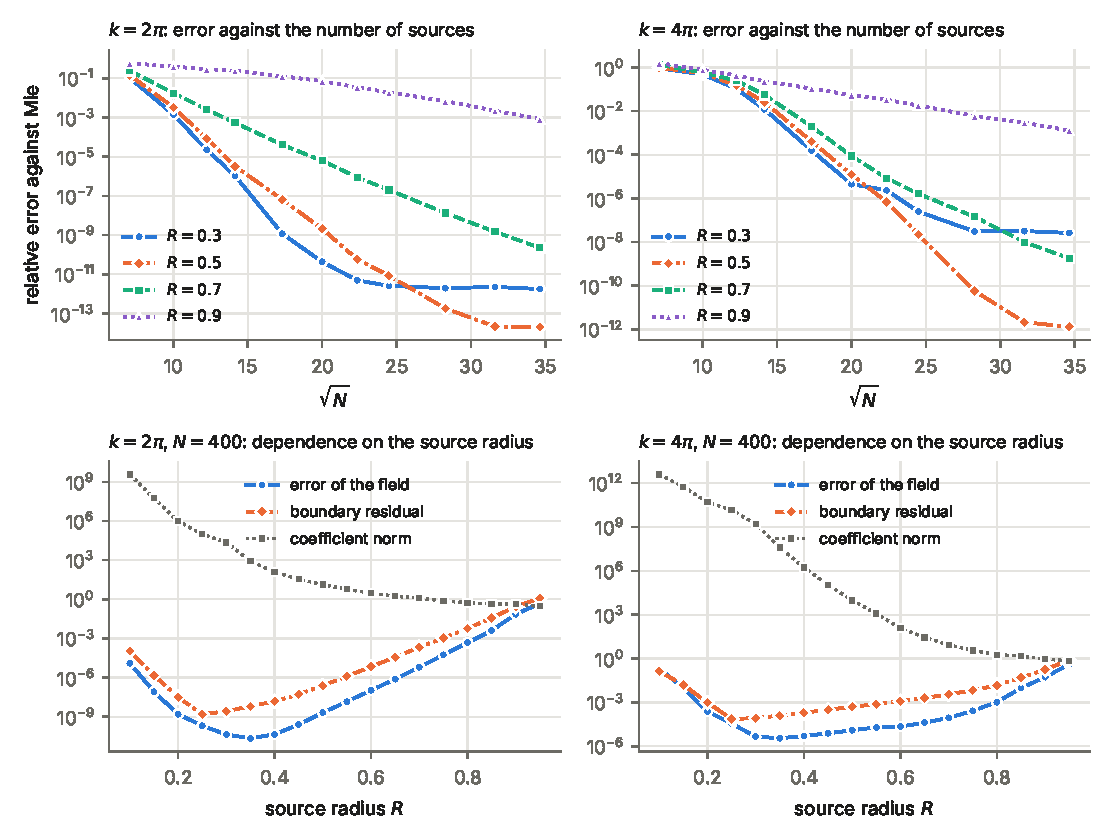
\includegraphics[width=\textwidth]{fig_sphere.pdf}
  \caption{Perfectly conducting unit sphere, error against the Mie series at $400$ points on $|\bx| = 1.5$. Top: error against $\sqrt{N}$ for four source radii $R$. Bottom: error, boundary residual and coefficient norm against $R$ for $N = 400$. Left: $k = 2\pi$. Right: $k = 4\pi$.}
  \label{fig:sphere}
\end{figure}

\subsection{Dependence on the wavenumber}

We repeated the experiment with $R = 0.5$ for $k = 4\pi$, $6\pi$ and $8\pi$, for which the sphere is four, six and eight wavelengths across. Interpolating between the runs, an error of $10^{-6}$ needs about $220$, $470$, $800$ and $1630$ sources at $k = 2\pi$, $4\pi$, $6\pi$ and $8\pi$. For the three larger spheres this is between $21$ and $28$ unknowns per square wavelength of surface. The number of unknowns thus grows in proportion to the surface area measured in wavelengths, as it must, and the constant is small. At $k = 8\pi$ the run with $1600$ sources takes $9$\,s. With more sources the error at this wavenumber stalls near $3\times10^{-9}$, because the coefficients grow as described above.

\subsection{Cost}
\label{sec:spherecost}

\autoref{tab:sphere} and \autoref{fig:costsphere} compare the MFS with Bempp. With $1200$ unknowns the MFS reaches an error of $2.0\times10^{-9}$ in $0.29$\,s. Bempp reaches $3.7\times10^{-3}$ with $9750$ unknowns in $19$\,s. Its error halves when the number of unknowns doubles, which is the rate of a lowest-order method on a surface approximated by flat triangles. Neither method uses the symmetry of the sphere.

The comparison is between a spectrally accurate method and a low-order one, and on a smooth body the outcome is not surprising. A boundary element method of high order on curved elements would converge much faster than Bempp does here. We include the sphere because it calibrates both codes against an exact solution.

\begin{table}[htbp]
  \centering
  \caption{Unit sphere, $k = 2\pi$: unknowns, wall time and error against the Mie series. MFS with $R = 0.5$; Bempp on quasi-uniform meshes.}
  \label{tab:sphere}
  \begin{tabular}{lrrl}
    \toprule
    Method & Unknowns & Time [s] & Error \\
    \midrule
\tablebody{sphere}
    \bottomrule
  \end{tabular}
\end{table}

\begin{figure}[htbp]
  \centering
  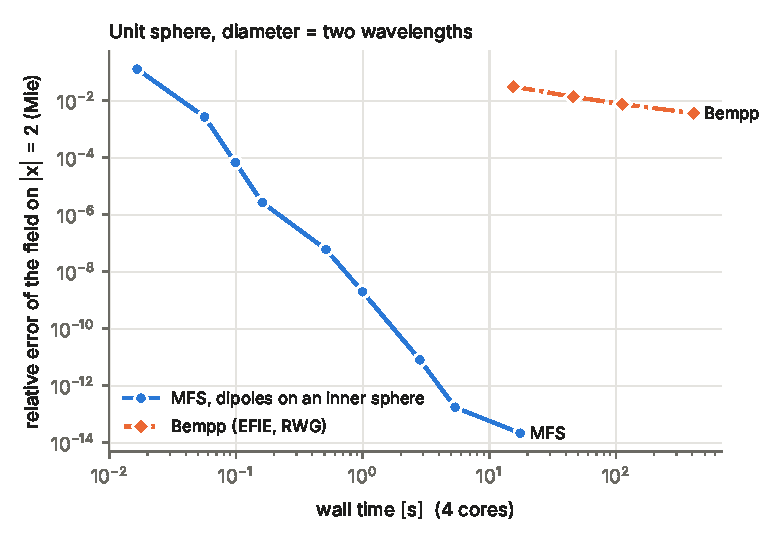
\includegraphics[width=0.62\textwidth]{fig_cost_sphere.pdf}
  \caption{Unit sphere, $k = 2\pi$: error against the Mie series as a function of wall time on four cores.}
  \label{fig:costsphere}
\end{figure}

\section{The torus}
\label{sec:torus}

The sphere is forgiving because its only singularity is a point. Our second smooth body is the torus
\begin{equation}
  \bigl(\rho - R\bigr)^2 + z^2 = a^2, \qquad \rho = \sqrt{x^2+y^2},
\end{equation}
with major radius $R = 1$ and minor radius $a = 0.5$, again at $k = 2\pi$. It is not convex, and it has no closed-form solution. Tori are standard test bodies for the MFS in acoustics \cite{cai2026}, and the MAS has been applied to them \cite{zaridze2004}. We use the torus to show that the layout of the sphere carries over to a ring-shaped conductor, and that the radius of the source surface is then bounded from below.

\subsection{Layout}

The sources are electric dipoles on the inner torus with the same centre circle and minor radius $a_s < a$. They are arranged on $n_s$ rings around the tube, with $n_\varphi$ equally spaced dipoles per ring. The collocation points lie on $2n_s$ rings of the surface with $n_\varphi$ points each, and each point is weighted by its area. Both sets are invariant under rotation by $2\pi/n_\varphi$ about the axis. The least-squares problem therefore splits exactly into $n_\varphi$ independent problems, one for each Fourier mode about the axis, and this holds for any incident wave. We solve the small problems one by one. The splitting is the one used by Liu and Barnett for acoustic scattering by axisymmetric bodies \cite{liu2016}. We checked it against the full matrix, and the two solutions agree to $8\times10^{-15}$.

\subsection{Where the source torus may be}

For the torus the continued field is not singular at a single point. Let $c = \sqrt{R^2-a^2}$. The circle $\rho = c$, $z = 0$ is the focal ring of the toroidal coordinate system in which the surface is a coordinate surface. It lies inside the tube, between the centre circle $\rho = R$ and the inner wall. We argue in \ref{app:torus} that the continued field is singular on the centre circle and on the focal ring. A source torus that is concentric with the tube encloses both only if
\begin{equation}
  a_s > R - \sqrt{R^2-a^2}.
  \label{eq:torusradius}
\end{equation}
As a fraction of $a$ the bound is $0.127$, $0.268$ and $0.5$ for $a/R = 0.25$, $0.5$ and $0.8$. A fat torus leaves little room.

We have not proved \eqref{eq:torusradius}, and we present it as a conjecture supported by two numerical tests. The first test fits the decay of the Fourier coefficients of the dipole density around a source circle, which gives the distance from the centre of the circle to the nearest singularity. For $a/R = 0.8$ the fitted distance is between $0.39$ and $0.40$ for four different incident waves and two wavenumbers, and the predicted value is $R - c = 0.40$. The second test is shown in \autoref{fig:torussources}. With a fixed number of sources, the norm of the coefficients stays of order one while $a_s$ satisfies \eqref{eq:torusradius} and grows by orders of magnitude below the bound. For $a/R = 0.8$ it is $3.6$ at $a_s/a = 0.5$ and $7\times10^{4}$ at $a_s/a = 0.4$. This is the behaviour that Barnett and Betcke prove for the disc (their Theorems 6 and 7 \cite{barnett2008}).

\begin{figure}[htbp]
  \centering
  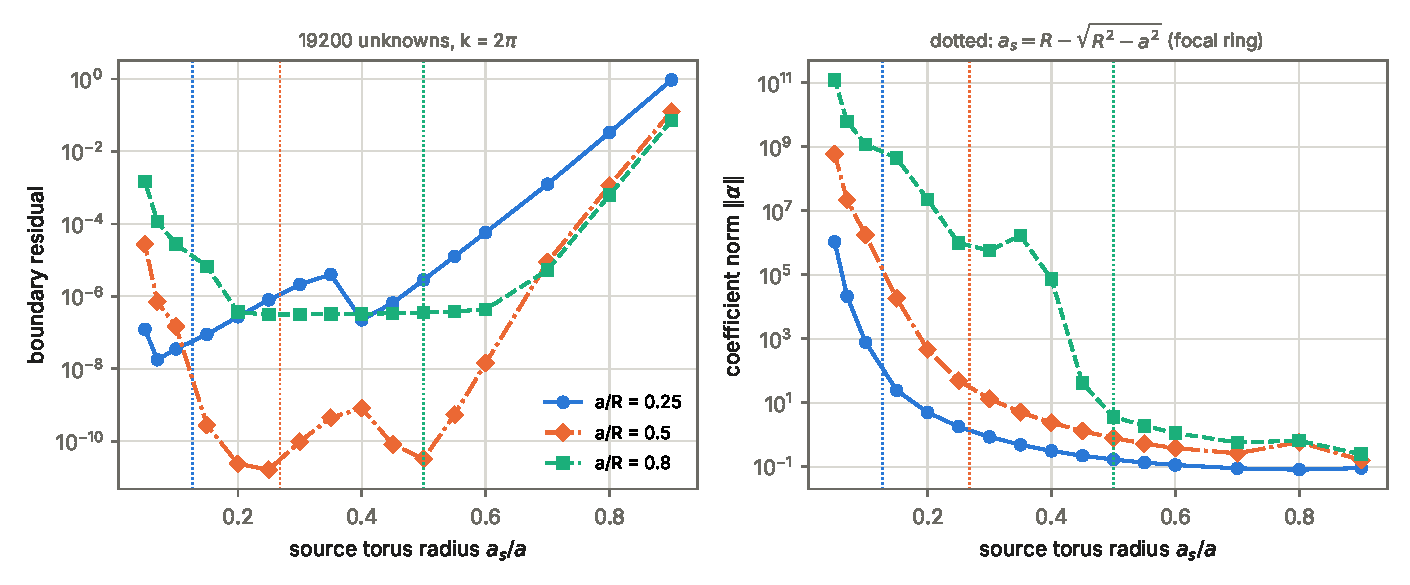
\includegraphics[width=\textwidth]{fig_torus_sources.pdf}
  \caption{Torus with $R = 1$ and three minor radii $a$, $k = 2\pi$, $19200$ unknowns. Boundary residual (left) and coefficient norm (right) against the radius of the source torus. The dotted lines mark the bound \eqref{eq:torusradius}.}
  \label{fig:torussources}
\end{figure}

\subsection{Results}

We take $a_s = 0.5\,a$, which satisfies \eqref{eq:torusradius} for $a/R = 0.5$. \autoref{tab:torus} lists the error of the scattered field against the finest MFS run, which has $40320$ unknowns, a boundary residual of $1.1\times10^{-10}$ and an optical mismatch of $9\times10^{-14}$. The error falls from $5.0\times10^{-3}$ with $1440$ unknowns to $7.3\times10^{-12}$ with $21120$ unknowns, and the finest of these runs takes $6.3$\,s. For a wave arriving obliquely, from the polar angle $60^\circ$ and the azimuth $25^\circ$, the boundary residual with $21120$ unknowns is $2.6\times10^{-10}$.

There is no exact solution to compare with. Bempp with $9600$ unknowns is $8.2\times10^{-3}$ away from the MFS field after $21$\,s. Its extinction cross-section approaches the MFS value $11.7526$ like the reciprocal of the number of unknowns, and extrapolation gives $11.7533$, a relative difference of $7\times10^{-5}$.

The MFS uses the rotational symmetry of the body and Bempp does not. To separate the two effects, \autoref{tab:torus} also lists the MFS with the full matrix. Without the symmetry the MFS needs $19$\,s for an error of $1.1\times10^{-4}$. A boundary element code for bodies of revolution would gain from the symmetry in the same way.

\begin{table}[htbp]
  \centering
  \caption{Torus, $R = 1$, $a = 0.5$, $k = 2\pi$, wave along the axis: unknowns, wall time and difference from the finest MFS run.}
  \label{tab:torus}
  \begin{tabular}{lrrl}
    \toprule
    Method & Unknowns & Time [s] & Error \\
    \midrule
\tablebody{torus}
    \bottomrule
  \end{tabular}
\end{table}

\section{Why an inner copy of the surface fails}
\label{sec:skeleton}

The layout of the two previous sections places the sources on a smaller copy of the surface. For the cube and the almond this layout does not converge.

\emph{Cube.} For the unit cube at $k = 2\pi$ we placed between $96$ and $600$ electric dipoles on the faces of a concentric inner cube. The error of the scattered field stays between $21\%$ and $30\%$ and does not decrease as sources are added (\autoref{sec:cube}).

\emph{Almond.} For the NASA almond at $1.19$\,GHz, our first layouts on an inner surface were unstable and failed a test with a known exterior solution. A confocal inner surface that resolves the rim gave a stable fit, but its boundary residual remained at $22\%$ with $1243$ sources.

Both failures have the same cause, and it is the rule quoted in the introduction: the sources must enclose the singularities of the continued field. We now locate these singularities for both shapes.

\subsection{Convex polyhedra}

For a polyhedron the continuation can be written down explicitly. Let $\Omega$ be a convex polyhedron. For each face $F$ let $C_F$ be the set of points of $\Omega$ that are closer to the plane of $F$ than to the plane of any other face. The cells $C_F$ fill $\Omega$, and their common walls form the interior medial surface $\mathcal{M}$ of the polyhedron, which we call its \emph{skeleton}. For the cube the skeleton consists of twelve triangles. Each triangle joins an edge to the centre and lies in the plane that bisects the two faces meeting at that edge.

\begin{theorem}
\label{thm:skeleton}
Let $\Omega$ be a convex perfectly conducting polyhedron with skeleton $\mathcal{M}$, and let $\Einc$ be an entire solution of Maxwell's equations. Then the scattered field outside $\Omega$ is the field radiated by an electric surface current $\bJ$ and a magnetic surface current $\bK$ on $\mathcal{M}$.
\end{theorem}

\begin{proof}
Let $(\bE^{t},\bH^{t})$ be the total field outside $\Omega$. Fix a face $F$ with unit normal $\bn$, let $\bx^*$ be the mirror image of $\bx$ in the plane of $F$, and let $P = I - 2\bn\bn^{\top}$. The reflected field
\begin{equation}
  \bE_F(\bx) = -P\,\bE^{t}(\bx^*), \qquad \bH_F(\bx) = P\,\bH^{t}(\bx^*)
\end{equation}
solves Maxwell's equations wherever $\bx^*$ lies outside $\Omega$. Since $\Omega$ is convex, its mirror image lies outside $\Omega$, so $(\bE_F,\bH_F)$ is defined in all of $\Omega$. On $F$ the total field satisfies $\bn\times\bE^{t} = 0$ and therefore $\bn\cdot\bH^{t} = 0$. Hence the reflected field has the same tangential traces on $F$ as the total field, and it continues the total field analytically across the open face. This is the image principle read backwards.

Define $\mathbf{V} = \bE^{t}$ outside $\Omega$ and $\mathbf{V} = \bE_F$ in each cell $C_F$. Then $\mathbf{V}$ solves Maxwell's equations away from $\mathcal{M}$, and $\mathbf{U} = \mathbf{V} - \Einc$ equals the scattered field outside $\Omega$ and satisfies the radiation condition. We apply the Stratton--Chu representation formula \cite{colton2013} to $\mathbf{U}$ on the two sides of $\mathcal{M}$. Small tubes around the edges and small balls around the vertices contribute nothing in the limit. The reason is that the field grows at most like $\rho^{-1/3}$ at distance $\rho$ from an edge and like $r^{\nu-1}$ with $\nu > 0$ at distance $r$ from a vertex \cite{meixner1972,costabel2000}. The reflected fields inherit the same growth. What remains is the field of the currents
\begin{equation}
  \bJ = \bn_{\mathcal{M}}\times[\bH], \qquad \bK = -\bn_{\mathcal{M}}\times[\bE]
  \label{eq:jumps}
\end{equation}
on $\mathcal{M}$, where $[\,\cdot\,]$ denotes the jump between the continuations from the two neighbouring cells.
\end{proof}

The theorem has three consequences for the method.
\begin{enumerate}
  \item Sources on the skeleton are sufficient, and nothing closer to the faces is needed.
  \item The skeleton contains the edges. A shrunk copy of the surface does not reach them and cannot represent the field. This is the stall at $21$--$30\%$.
  \item Both currents in \eqref{eq:jumps} are non-zero in general, so both electric and magnetic dipoles are needed. With electric dipoles alone, our edge sources stalled at an error of $5\%$.
\end{enumerate}
The densities $\bJ$ and $\bK$ are smooth on each wall of the skeleton and become singular only towards the edges and vertices. This is where the sources must cluster.

\begin{remark}
The statement has a relative in potential theory. Gustafsson \cite{gustafsson1998} showed that a convex polyhedron of uniform density has the same exterior Newtonian potential as a measure supported on finitely many planes inside it, which reaches the boundary only at edges and corners. \autoref{thm:skeleton} is the corresponding statement for scattering by a conductor. To our knowledge it has not been stated in this form. The proof uses convexity. For a non-convex polyhedron the mirror image of the body can re-enter the body, and the statement does not hold as it stands.
\end{remark}

\subsection{Smooth thin bodies}

For a smooth surface there is no reflection formula, but the location of the singularities is known in simple cases. For an ellipse in two dimensions the continued field is singular at the two foci \cite{millar1971,barnett2008}. Every cross-section of the almond is an ellipse with axis ratio $3:1$, whose foci lie at the fraction $\sqrt{1-1/9}\approx0.943$ of the semi-major axis. We therefore expect the singularities of the continued field of the almond on the curve traced by these foci in the mid-plane. This \emph{focal curve} runs within $6\%$ of the rim. A shrunk copy of the surface that stays outside the focal curve would have to lie within $6\%$ of the rim itself, where it is too close to the surface to be useful.

This is the standard continuation argument applied section by section, and it is not a proof for the three-dimensional body. Our evidence is numerical. Sources on the mid-plane that cluster towards the focal curve converge (\autoref{sec:almond}), and sources on surfaces that leave the focal curve outside do not.

The skeleton of the cube and the mid-plane of the almond play the same role. In both cases the sources are placed on a surface inside the body that the continued field cannot cross, and they cluster towards the part of that surface which touches or approaches the boundary.

\section{The cube: edge sources and singular tails}
\label{sec:cube}

We now construct sources for the unit cube $[-\tfrac12,\tfrac12]^3$ at $k = 2\pi$, so that the side is one wavelength. By \autoref{thm:skeleton} the sources belong on the twelve bisector planes of the edges, and they must resolve current densities that are singular at the edges and vertices.

\subsection{Sources}

The layout has four parts (\autoref{fig:cubelayout}).

\emph{Base points.} A grid of $n_b\times n_b$ electric dipoles on each face of the inner cube at depth $0.2$ below the faces represents the smooth part of the field.

\emph{Edge lines.} For each edge we choose depths that decrease geometrically,
\begin{equation}
  d = 0.2\,q^{\,j}, \qquad j = 0,1,\dots, \qquad \text{down to } d_J = 0.2\cdot 2^{-J},
  \label{eq:depths}
\end{equation}
and place at each depth a line parallel to the edge, on the bisector plane, at distance $d$ from the edge. We call $J$ the level of the layout and $d_J$ its deepest depth. We use two ratios: $q = 1/2$, which gives one line for each octave of depth, and $q = 2^{-1/2}$, which gives two. In two dimensions a lightning solver would place one point source at each depth \cite{gopal2019siam,ginn2023}. In three dimensions a row of point sources along the line does not work: at depth $d$ the points would have to be spaced by about $d$, which requires $1/d$ of them. We therefore let each line carry a continuous dipole density. With $t\in[-(\tfrac12-d),\tfrac12-d]$ the coordinate along the line at depth $d$, we introduce the stretched variable
\begin{equation}
  u(t) = \frac{1}{\lambda}\log\frac{\tfrac12+t}{\tfrac12-t}, \qquad \lambda = \log\frac{1-d}{d},
\end{equation}
which maps the line to $[-1,1]$ and resolves every scale between $d$ and the length of the edge near both vertices. The density is a vector polynomial in $u$,
\begin{equation}
  \ba(t) = \sum_{l=0}^{n-1}\ba_l\,P_l\bigl(u(t)\bigr), \qquad n = n_0 + \lceil 2\log(1/d)\rceil,
  \label{eq:modes}
\end{equation}
with Legendre polynomials $P_l$ and unknown coefficients $\ba_l\in\mathbb{C}^3$. Each line exists twice, once with electric and once with magnetic dipoles. A line at depth $10^{-3}$ thus costs about $20$ modes, where a row of points would need a thousand. The line integrals are evaluated by the quadrature of \ref{app:lines}.

\emph{Vertex points.} On the body diagonal through each vertex we place an electric and a magnetic point dipole at each of the same distances $d$ from the vertex.

\emph{Tails.} The deepest free line lies at the depth $d_J$. The current sheet of \autoref{thm:skeleton} continues below this depth, and cutting it off leaves an error that decays only like $d_J^{0.55}$ in our experiments. We therefore continue the lines at the depths $d_J2^{-i}$, $i = 1,\dots,9$. These lines are not free. They carry the modes of the line at $d_J$, multiplied by the fixed weights $2^{-ie}$, and the remainder of the geometric series below the last depth is added to the last line. The exponent $e$ depends on the component of the current. \autoref{tab:edgeexp} lists the four exponents, which follow from the edge expansion of the field (\ref{app:edge}). The tail of an edge adds two components of $n$ modes for each kind of dipole, where $n$ is the number of modes of the deepest free line. The component normal to the bisector plane vanishes and adds no unknowns. The vertex points are continued in the same way along the diagonal, with the exponents $e = \nu+2 = 2.454$ for the electric and $e = \tau+2 = 2.840$ for the magnetic dipoles (\ref{app:cone}).

\begin{table}[htbp]
  \centering
  \caption{Exponents of the edge tail. The current density on the bisector half-plane behaves like $\rho^{e-1}$ at depth $\rho$ below the edge.}
  \label{tab:edgeexp}
  \begin{tabular}{llll}
    \toprule
    Current & Component & Density & Tail exponent $e$ \\
    \midrule
    electric & along the edge & $\rho^{-1/3}$ & $2/3$ \\
    electric & along the bisector & $\rho^{2/3}$ & $5/3$ \\
    magnetic & along the edge & $\rho^{1/3}$ & $4/3$ \\
    magnetic & along the bisector & $\rho^{4/3}$ & $7/3$ \\
    \bottomrule
  \end{tabular}
\end{table}

\begin{figure}[htbp]
  \centering
  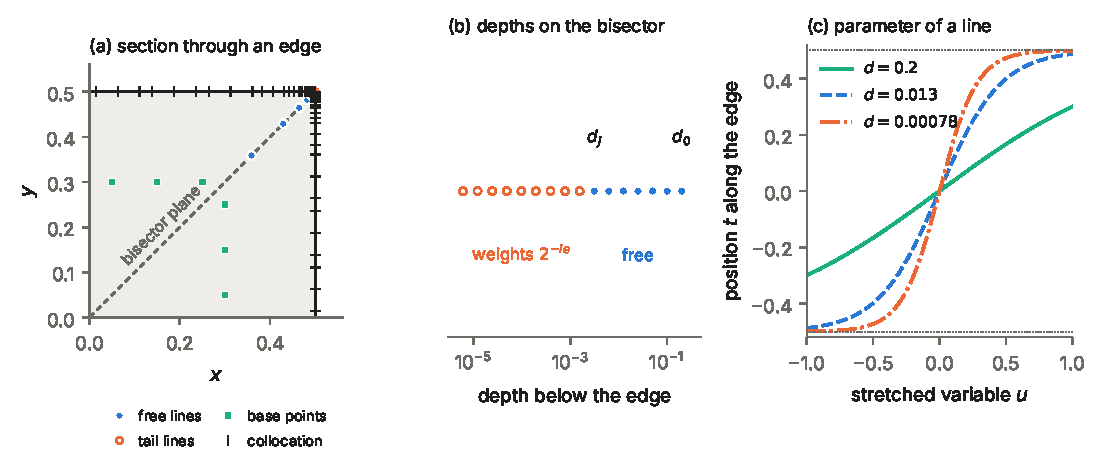
\includegraphics[width=0.9\textwidth]{fig_cube_layout.pdf}
  \caption{Source layout of the cube. (a) Cross-section through the middle of an edge: the lines, seen end on, sit on the bisector plane at the depths \eqref{eq:depths}; base points lie on an inner cube; collocation nodes on the two faces are graded towards the edge. (b) The depths on a logarithmic scale: free lines down to $d_J$, then the tail with fixed weights. (c) The stretched variable $u$ along a line, which clusters the modes towards the two vertices as the depth decreases.}
  \label{fig:cubelayout}
\end{figure}

\subsection{Collocation and weights}

The collocation points on each face form a tensor grid. In each direction the nodes are Gauss--Legendre points on panels that halve in length towards both edges until they are shorter than the deepest depth $d_J$. Panels in the interior are no longer than $h_{\max}$. We use three nodes per panel for $q = 1/2$ and four for $q = 2^{-1/2}$. The fit needs enough equations at every scale, and with too few it fails without any sign in the residual at the collocation points. With two nodes per panel and $q = 1/2$ the error of the field at $J = 5$ is $85\%$. With three nodes and $q = 2^{-1/2}$ it exceeds $90\%$ at $J = 6$. In both cases the optical mismatch, $0.35$ and $0.5$, reveals the failure.

The rows are weighted by
\begin{equation}
  w_i = A_i\,\rho_i^{2\beta}, \qquad \beta = \tfrac12,
\end{equation}
where $A_i$ is the area represented by the point and $\rho_i$ its distance to the nearest edge. Without the factor $\rho_i^{2\beta}$ the fit spends its effort on the edge singularity of the residual, and the far field is worse. Values of $\beta$ between $1/3$ and $3/4$ give similar results.

All resolution parameters must grow together. Refining the depth alone leaves other limits in place, and the error then stalls near $10^{-3}$. We use one family indexed by the level $J$ for each ratio $q$: $n_0 = \max(4, 2J-4)$, and $(n_b, h_{\max}) = (4, 0.25)$ for $J\le5$ and $(6, 0.15)$ for $J\ge6$.

\subsection{Symmetry}

The cube and the layout are symmetric under the three mirrors $x\to-x$, $y\to-y$ and $z\to-z$. Any incident field is the sum of eight parts of definite parity under the three mirrors, and each part is scattered into a field of the same parity. A part needs only the sources of one octant, with the modes of each line restricted to one parity, and collocation points in one octant. The eight matrices are signed sums of the same reflected blocks, so the line integrals are computed once. Each parity class has its own factorisation, which then serves every incident wave. Our standard wave excites two classes. A general wave excites all eight.

\subsection{Results}

\autoref{tab:cube} lists the results for the standard wave and both depth ratios. The reference is the run with two depths per octave at level $J = 11$.

\emph{Two depths per octave.} The difference between successive levels falls from $9.0\times10^{-3}$ between $J = 3$ and $4$ to $1.5\times10^{-5}$ between $J = 10$ and $11$, by a factor of $2.3$ to $2.9$ per level. The optical mismatch falls with it, from $3.1\times10^{-3}$ to $1.8\times10^{-6}$. If the decay continues at the same rate, the error of the reference itself is about $10^{-5}$. The entries of \autoref{tab:cube} are differences from the reference, so the last of them are uncertain by this amount. The result is insensitive to the other parameters. At $J = 9$ the field changes by less than $3\times10^{-6}$ when the number of modes is raised, the tails are lengthened from $9$ to $14$ lines, a second vertex exponent is added, the base grid is refined to $n_b = 8$ with $h_{\max} = 0.1$, or the collocation grid is replaced by one with three nodes per panel and panels that shrink by $2^{-1/2}$. Only the weight exponent $\beta$ has a visible effect: $\beta = 0.3$ and $\beta = 0.7$ change the field by $6\times10^{-5}$ and $2\times10^{-5}$, which is the size of the remaining error.

\emph{One depth per octave.} This layout has about $60\%$ of the unknowns and takes between $30\%$ and $60\%$ of the time. Down to level $J = 7$ its errors equal those of the denser layout to within $20\%$. Then it stalls: the error is $1.7\times10^{-4}$ at $J = 8$ and $1.5\times10^{-4}$ at $J = 9$. Deeper levels bring no gain. With the finer grid $(n_b, h_{\max}) = (8, 0.1)$ the errors at the levels $9$ to $12$ are between $1.3\times10^{-4}$ and $1.8\times10^{-4}$. With the grid of the table they rise again, to $2.9\times10^{-4}$ at $J = 10$: the coarser grid in the interior of the faces no longer suffices. The matrices are well conditioned, so this is a limit of approximation and not of rounding: one line per octave cannot represent the current sheet on the bisector plane more accurately. The two-dimensional analogue behaves in the same way. For the unit square in the polarisation with the stronger corner singularity, with point sources on the bisectors of the corners at depths down to $10^{-9}$, the error of the far field is $8\times10^{-5}$ for $q = 1/2$, $6\times10^{-6}$ for $q = 0.6$ and $10^{-9}$ for $q = 2^{-1/2}$. A fixed ratio gives a fixed attainable accuracy. We therefore regard $q = 1/2$ as the economical choice for errors down to $2\times10^{-4}$ and $q = 2^{-1/2}$ as the choice below.

\begin{table}[htbp]
  \centering
  \caption{Unit cube, $k = 2\pi$, standard wave. MFS with edge sources and tails, with one and with two source depths per octave: unknowns and equations per parity class (two classes are solved), wall time, difference from the run with two depths per octave at $J = 11$, and optical mismatch.}
  \label{tab:cube}
  \small
  \begin{tabular}{lrrrrll}
    \toprule
    Depths & $J$ & Unknowns & Equations & Time [s] & Error & Optical \\
    \midrule
\tablebody{cube_mfs}
    \bottomrule
  \end{tabular}
\end{table}

\emph{The tails are essential.} With one depth per octave and the same edge lines but without the tails, the error is $5.4\times10^{-2}$, $2.5\times10^{-2}$ and $1.1\times10^{-2}$ for $J = 4$, $6$ and $8$. At $J = 8$ the tails reduce the error by a factor of $64$ and add $9\%$ to the unknowns. \autoref{fig:edgeresidual} shows where the gain comes from. Without the tail the boundary residual near an edge is of order one at all distances below the deepest free depth $d_J$. With the tail it is one to two orders of magnitude smaller between the last tail line, at $d_J/512$, and $d_J$. Closer to the edge than the last tail line it grows again, on a strip whose area is negligible. Plain MFS with sources on an inner cube stays above $21\%$ (\autoref{fig:costcube}).

\begin{figure}[htbp]
  \centering
  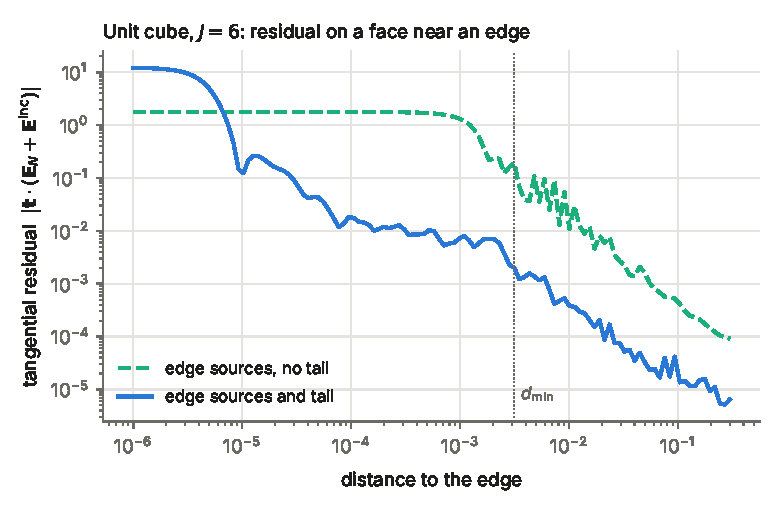
\includegraphics[width=0.62\textwidth]{fig_edge_residual.pdf}
  \caption{Unit cube, $J = 6$, one depth per octave: tangential residual on a face as a function of the distance to an edge, away from the vertices, with and without the tail. The dotted line marks the deepest free depth $d_J$.}
  \label{fig:edgeresidual}
\end{figure}

\emph{An independent reference.} Since no exact solution exists, we computed the same field with Bempp on meshes graded towards the edges (\ref{sec:bempp}). With the quadrature orders $8$ and $10$ and $10368$, $14112$, $18432$ and $28800$ unknowns, the boundary element field differs from the MFS reference by $2.0\times10^{-4}$, $1.5\times10^{-4}$, $1.2\times10^{-4}$ and $1.0\times10^{-4}$. The extinction cross-sections of the meshes with $7200$, $10368$ and $14112$ unknowns are $2.92745$, $2.92762$ and $2.92771$, with the extrapolated value $2.92786$. The MFS gives $2.92793$, $2.92796$ and $2.92798$ at $J = 9$, $10$ and $11$. The two methods thus agree to $1.0\times10^{-4}$ in the field and to $4\times10^{-5}$ in the cross-section. Below that level the only reference for the MFS is its own convergence.

\subsection{Cost}
\label{sec:cubecost}

Our MFS solver uses the three mirror planes of the cube. Bempp does not use the symmetry of a body. To compare the two methods on an equal footing we added the symmetry to the boundary element computation ourselves (\ref{sec:bempp}). Only the rows of the matrix that belong to one octant are assembled, the columns are folded with a symmetrised basis, and each parity class is solved by a small LU factorisation. The result is the Galerkin solution on the full mesh, up to the asymmetry of the quadrature rules. With the symmetry the boundary element solution is obtained $3.5$ to $8$ times faster, and meshes with up to $28800$ unknowns fit into memory. \autoref{tab:cubebem} lists the boundary element results with both times, and \autoref{fig:costcube} shows the error of all methods against the wall time. All errors are differences from the MFS reference.

On quasi-uniform meshes Bempp converges slowly, because the edge singularity limits the rate: $13302$ unknowns give an error of $1.9\times10^{-3}$. Grading the mesh towards the edges helps considerably. With the default quadrature the graded meshes stall near $8\times10^{-4}$. With the orders $6$ and $8$ they reach $2.9\times10^{-4}$ with $10368$ unknowns. The most accurate boundary element run, with the orders $8$ and $10$ and $28800$ unknowns, gives $1.0\times10^{-4}$ in $69$\,s. Beyond $14112$ unknowns the convergence slows, from $1.5\times10^{-4}$ to $1.2\times10^{-4}$ and $1.0\times10^{-4}$, probably because the triangles at the edges become thin.

\begin{table}[htbp]
  \centering
  \caption{Unit cube, standard wave: Bempp on quasi-uniform meshes and on meshes graded towards the edges, for three choices of the quadrature orders (regular/singular). Unknowns, difference from the MFS reference, and wall time without and with the mirror symmetry of the cube.}
  \label{tab:cubebem}
  \small
  \begin{tabular}{llrlrr}
    \toprule
    Mesh & Quadrature & Unknowns & Error & \multicolumn{2}{c}{Time [s]} \\
         &            &          &       & no symmetry & symmetry \\
    \midrule
\tablebody{cube_bem}
    \bottomrule
  \end{tabular}
\end{table}

\begin{figure}[htbp]
  \centering
  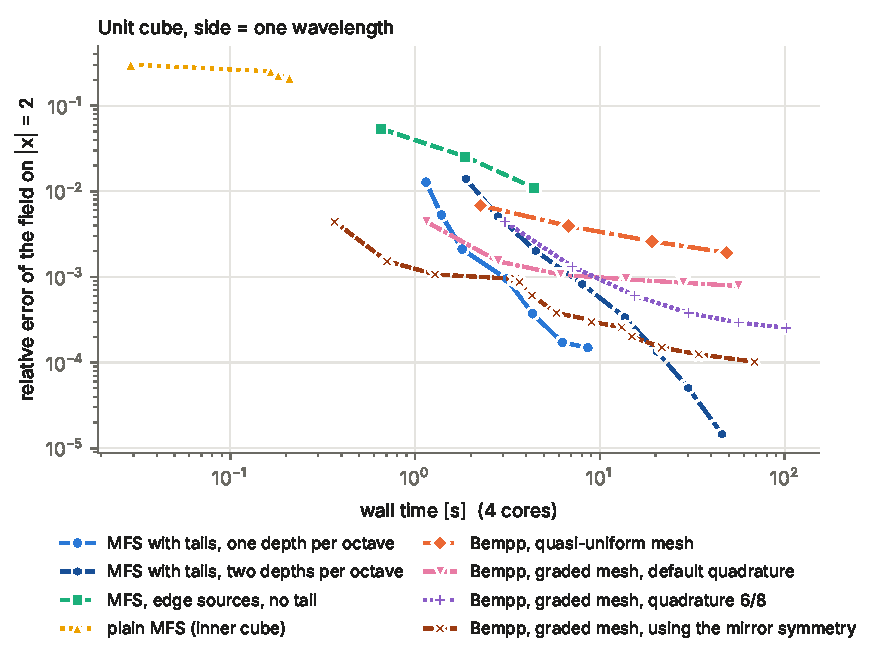
\includegraphics[width=0.78\textwidth]{fig_cost_cube.pdf}
  \caption{Unit cube, $k = 2\pi$, standard wave: difference from the MFS reference against wall time on four cores, for the MFS with tails (one and two depths per octave), the MFS without tails, plain MFS, and Bempp on quasi-uniform and graded meshes, without and with the mirror symmetry (for the latter, the best quadrature setting at each time).}
  \label{fig:costcube}
\end{figure}

With the symmetry used by both methods the comparison is as follows. Down to an error of $5\times10^{-4}$ the boundary element method is faster. It is fastest there with the default quadrature and milder gradings, which are not in \autoref{tab:cubebem}. With $g = 1.5$ it needs $1.5$\,s for $1.2\times10^{-3}$, and with $g = 1.75$ it needs $2.6$\,s for $5.4\times10^{-4}$, where the MFS needs $3.1$\,s for $9.5\times10^{-4}$. Below $4\times10^{-4}$ the MFS is faster. In $4.3$\,s it reaches $3.7\times10^{-4}$, where the boundary element method needs $5.0$\,s for $4.3\times10^{-4}$ and $5.8$\,s for $3.8\times10^{-4}$.
%% TODO (authors): add the rows for g = 1.5 and 1.75 to Table 5 and Figure 6, after a full scan of the grading; see NOTES.md item 58. The MFS needs $6.3$\,s for $1.7\times10^{-4}$ and $8.6$\,s for $1.5\times10^{-4}$, where the boundary element method needs $15$\,s for $2.0\times10^{-4}$ and $22$\,s for $1.5\times10^{-4}$. The smallest error of the boundary element method, $1.0\times10^{-4}$, takes $69$\,s. The MFS with two depths per octave reaches $1.3\times10^{-4}$ in $20$\,s, $5.0\times10^{-5}$ in $30$\,s and $1.5\times10^{-5}$ in $46$\,s.

Against Bempp as it is distributed, without the symmetry, the MFS is faster from $10^{-3}$ downwards: by a factor of two at $10^{-3}$ ($3.1$\,s against $6.1$\,s), of seven at $4\times10^{-4}$ ($4.3$\,s against $30$\,s) and of fifteen at $2\times10^{-4}$ ($6.3$\,s against $97$\,s).

One qualification remains. The MFS is not economical in unknowns. At $J = 6$ with one depth per octave the eight classes together have about $10^4$ unknowns for an error of about $10^{-3}$, which the graded boundary element mesh reaches with fewer than $5000$. What the MFS offers on the cube is its rate of convergence: the error falls by a factor of about $2.5$ per level, for $20$ to $50\%$ more unknowns, and it does not flatten where the boundary element method does.

\subsection{A general incident wave}
\label{sec:cubeoblique}

A wave from a general direction excites all eight classes. We tested the wave that arrives from the polar angle $60^\circ$ and the azimuth $25^\circ$, with its polarisation rotated by $35^\circ$ from the plane of incidence. For the MFS the assembly is shared between the classes, and eight factorisations are needed instead of two. For the boundary element method with symmetry the cost hardly changes. \autoref{tab:cubeoblique} compares the two. The reference is the run with two depths per octave at $J = 10$ for this wave.

The MFS converges as for the standard wave. With one depth per octave the error falls from $6.2\times10^{-3}$ at $J = 4$ to $1.9\times10^{-4}$ at $J = 9$, and the cost is $1.4$ to $2.3$ times that of the standard wave. With the symmetry used by both methods, the boundary element method is faster down to $4\times10^{-4}$: it needs $5.0$\,s for $5.2\times10^{-4}$, where the MFS needs $8.8$\,s. Below that the two are level: $15$\,s against $14$\,s at $2.7\times10^{-4}$, $24$\,s for $2.0\times10^{-4}$ against $20$\,s for $1.9\times10^{-4}$, and $91$\,s for $1.3\times10^{-4}$ against $65$\,s for $1.4\times10^{-4}$. Against Bempp without the symmetry the MFS is faster below $10^{-3}$, for example $8.8$\,s against $30$\,s at $5\times10^{-4}$.

\begin{table}[htbp]
  \centering
  \caption{Unit cube, oblique wave: MFS with eight parity classes, and Bempp on graded meshes without and with the mirror symmetry. Unknowns (for the MFS, all classes together), wall time and difference from the MFS run with two depths per octave at $J = 10$. ``One depth'' and ``two depths'' refer to the number of source depths per octave. At $J = 8$ the run with two depths per octave solves the classes in groups to save memory, which repeats part of the assembly.}
  \label{tab:cubeoblique}
  \small
  \begin{tabular}{lrrl}
    \toprule
    Method & Unknowns & Time [s] & Error \\
    \midrule
\tablebody{cube_oblique}
    \bottomrule
  \end{tabular}
\end{table}

\subsection{A cube of two wavelengths}
\label{sec:cubek}

All results so far are for a side of one wavelength. We repeated the computation for the standard wave at $k = 4\pi$, where the side is two wavelengths. The layout is the same except for two parameters that follow the wavelength. The interior collocation panels are half as long, so $h_{\max}$ is halved, and each line carries four more modes, so $n_0$ is raised by four. The line quadrature uses more nodes (\ref{app:lines}). \autoref{tab:cubek} lists the results. The reference is the run with two depths per octave at $J = 10$, whose optical mismatch is $4.5\times10^{-6}$.

The method converges as at one wavelength. With two depths per octave the error falls from $2.2\times10^{-3}$ at $J = 5$ to $4.5\times10^{-5}$ at $J = 9$, by a factor of $2.4$ to $3.3$ per level. The layouts have $15$ to $30\%$ more unknowns than at $k = 2\pi$. The boundary element solution approaches the MFS field. With the quadrature orders $8$ and $10$ and $10368$, $18432$ and $28800$ unknowns it differs from the reference by $1.0\times10^{-3}$, $4.1\times10^{-4}$ and $2.4\times10^{-4}$.

With the symmetry used by both methods, the boundary element method is faster down to an error of $10^{-3}$. With the grading $g = 1.5$ and the default quadrature it needs $4.4$\,s for $1.1\times10^{-3}$, where the MFS needs $6.8$\,s. Below that the MFS is faster: $9.3$\,s against $20$\,s at $5\times10^{-4}$, and $13$\,s for $2.2\times10^{-4}$ against $74$\,s for $2.4\times10^{-4}$. The numbers of unknowns grow at different rates. For an error near $4\times10^{-4}$ the boundary element mesh needs $18432$ unknowns in place of the $7200$ at one wavelength. The MFS needs $1917$ per class in place of $1605$.

For the oblique wave of \autoref{sec:cubeoblique} the picture at two wavelengths is similar. Here the reference is the MFS run with two depths per octave at $J = 9$. The boundary element method is faster down to $1.2\times10^{-3}$, with $7.1$\,s for $1.3\times10^{-3}$ against $12$\,s for $1.5\times10^{-3}$. Below that the MFS is faster: $18$\,s for $6.4\times10^{-4}$ against $25$\,s for $6.5\times10^{-4}$, and $28$\,s for $2.7\times10^{-4}$ against $113$\,s for $3.5\times10^{-4}$.

\begin{table}[htbp]
  \centering
  \caption{Unit cube at $k = 4\pi$ (side of two wavelengths), standard wave: MFS with one and two source depths per octave, and Bempp on graded meshes with the mirror symmetry. Unknowns (for the MFS, per parity class; two classes are solved), wall time and difference from the MFS run with two depths per octave at $J = 10$. That run solves the two classes one after the other to save memory.}
  \label{tab:cubek}
  \small
  \begin{tabular}{lrrl}
    \toprule
    Method & Unknowns & Time [s] & Error \\
    \midrule
\tablebody{cube_k2}
    \bottomrule
  \end{tabular}
\end{table}

\section{The almond: skeleton sources and a tip tail}
\label{sec:almond}

The NASA almond \cite{woo1993} is a standard target for radar cross-section codes. It is a smooth body of length $L = 0.2524$\,m ($9.936$\,in) with a rounded rear and a sharp tip. Every cross-section is an ellipse with axis ratio $3:1$. We place the almond with its long axis along $x$, the tip at positive $x$ and its mid-plane in $z = 0$. It is symmetric under the mirrors $y\to-y$ and $z\to-z$.

\subsection{Sources}

By \autoref{sec:skeleton} the sources lie on the mid-plane and cluster towards the focal curve, which runs at the fraction $\eta_F = 0.943$ of the half-width (\autoref{fig:almondlayout}). They are point dipoles arranged in rows. A row follows the outline of the mid-plane section at a fixed fraction $\eta$ of the half-width. We use $n_{\mathrm{mid}}$ rows in the middle of the section and $J+1$ rows at
\begin{equation}
  \eta_j = \eta_F - 2\,(1-\eta_F)\,2^{-j}, \qquad j = 0,\dots,J,
\end{equation}
which approach the focal curve geometrically from the inside. Along a row the spacing of the sources is a fixed multiple $s$ of the local distance to the surface. The collocation points on the surface follow the same rule, so that sources and collocation points refine together towards the rim. We write $n_{\mathrm{mid}}{:}J$ for a layout.

A source on a mirror plane of a field of definite parity keeps only three of its six dipole components. For fields that are even under $z\to-z$ these are the electric components $a_x$, $a_y$ and the magnetic component $m_z$. For odd fields they are $a_z$, $m_x$ and $m_y$. Each source therefore carries three unknowns. As for the cube, an incident wave is split into its parts of definite parity under the two mirrors. Each of the four classes is solved with the sources and collocation points of one quarter of the body.

\begin{figure}[htbp]
  \centering
  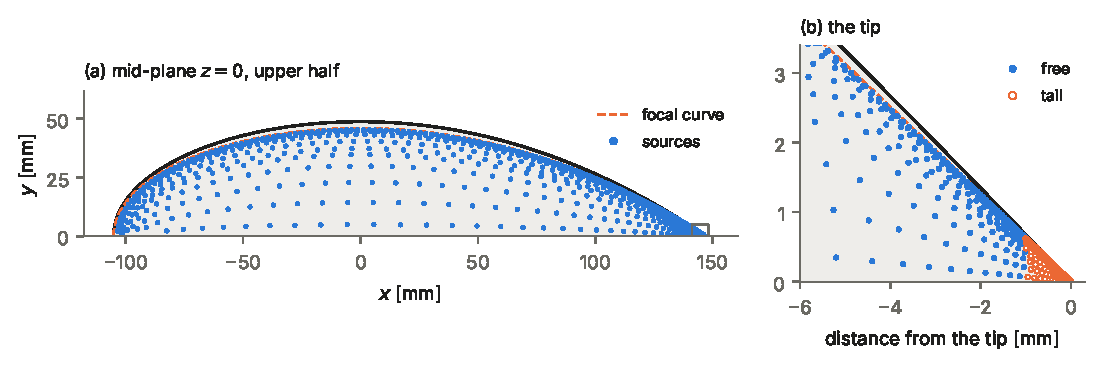
\includegraphics[width=0.9\textwidth]{fig_almond_layout.pdf}
  \caption{Source layout of the almond in the mid-plane $z = 0$ (one half shown). The rows of point dipoles cluster towards the focal curve (dashed), which runs within $6\%$ of the rim, and continue into the tip as a tail.}
  \label{fig:almondlayout}
\end{figure}

\subsection{The tip}

The focal curve reaches the surface at the tip, which is the vertex of an elliptic cone with half-angles $34.09^\circ$ and $12.71^\circ$. The field of a conducting cone behaves like $r^{\nu-1}$ at distance $r$ from the vertex. For this cone the smallest exponent is $\nu = 0.29959$ (\ref{app:cone}), so the electric field grows like $r^{-0.70}$. This singular term belongs to the class that is even under both mirrors, which is the class that drives current along the axis into the tip. In the other three classes all exponents exceed $0.87$.

The free source rows stop $1$\,mm from the tip. For the class that is even under both mirrors this cut-off leaves a boundary residual of $19\%$, half of it within $1$\,mm of the tip. The cross-section at oblique angles is then wrong by up to $1.2$\,dB. Adding sources does not help. The remedy is the tail of \autoref{sec:cube}. Each row is continued to within $10^{-4}$\,mm of the tip with the same spacing rule. The continued dipoles of a row are tied together with the weights $(r/r_{\mathrm{cut}})^{e}$, where $e = \nu+2$ for electric and $e = \tau+2$ for magnetic dipoles. With the tail and the spacing $s = 0.5$ the residual of this class falls to $0.23\%$, and with $s = 0.4$ to $0.034\%$. The other classes are converged at $s = 0.7$.

Before we computed the exponents of the cone we had fitted a set of four exponents between $2.2$ and $3.0$. The single computed value $e = 2.29959$ gives the same residual, and the fitted set is no longer needed.

\subsection{Nose-on incidence at 1.19 GHz}

We first consider the wave that travels along $-x$ towards the tip, polarised along $y$, at $1.19$\,GHz, where the almond is one wavelength long. \autoref{tab:almond} and \autoref{fig:costalmond} show the difference from the finest layout, $8{:}5$ with $4791$ unknowns. This reference is itself converged: a closer spacing along the rows ($s = 0.5$), a finer collocation grid, and twice as many rows towards the focal curve each change its field by less than $10^{-5}$. The layouts $5{:}2$ and $6{:}3$ reach $2.8\times10^{-4}$ and $5.6\times10^{-5}$ in $2.1$ and $3.2$\,s. Bempp reaches $3.0\times10^{-3}$ with $9558$ unknowns in $19$\,s, and its error is inversely proportional to the number of unknowns. At an error of one per cent the two methods take about the same time, one second. The MFS uses the two mirror symmetries of this wave, which Bempp does not.

\begin{table}[htbp]
  \centering
  \caption{NASA almond, $1.19$\,GHz, nose-on incidence: unknowns, wall time and difference from the finest MFS layout.}
  \label{tab:almond}
  \begin{tabular}{lrrl}
    \toprule
    Method & Unknowns & Time [s] & Error \\
    \midrule
\tablebody{almond}
    \bottomrule
  \end{tabular}
\end{table}

\begin{figure}[htbp]
  \centering
  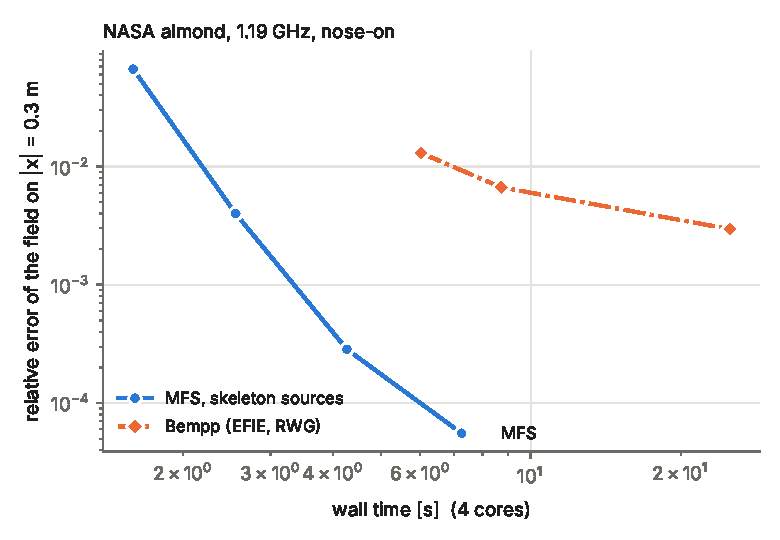
\includegraphics[width=0.62\textwidth]{fig_cost_almond.pdf}
  \caption{NASA almond, $1.19$\,GHz, nose-on incidence: difference from the finest MFS layout against wall time on four cores.}
  \label{fig:costalmond}
\end{figure}

\subsection{Monostatic radar cross-section}

The quantity of practical interest is the monostatic cross-section as a function of the azimuth in the plane of the almond, for the polarisations HH (electric field in the plane) and VV (electric field along $z$). HH needs the two classes that are even in $z$ and VV the two that are odd. The factorisation of a class serves all look angles. One frequency, with $361$ look angles and both polarisations, takes $66$\,s with the layout $6{:}3$.

We compare with the Austin RCS Benchmark Suite \cite{kelley2020}, which provides measurements of this almond and a reference simulation on a fine mesh at $3.5$, $5.125$, $7$ and $10.25$\,GHz. At the highest frequency the almond is $8.6$ wavelengths long. \autoref{fig:almondbench} shows the three sets of curves, and \autoref{tab:almondbench} lists the mean absolute difference in decibels over the $361$ look angles. The MFS differs from the reference simulation by $0.04$ to $0.14$\,dB for HH and by $0.01$ to $0.02$\,dB for VV. Both simulations differ from the measurements by $0.6$ to $1.8$\,dB, and the two distances agree to within $0.07$\,dB in every case.
%% TODO: quote the measurement uncertainty from Kelley et al. once the paper is at hand.

\begin{table}[htbp]
  \centering
  \caption{NASA almond, monostatic cross-section: mean absolute difference in dB between the MFS (layout $6{:}3$) and the reference simulation of the Austin benchmark \cite{kelley2020}, over $361$ look angles.}
  \label{tab:almondbench}
  \begin{tabular}{lrrrr}
    \toprule
    Frequency [GHz] & 3.5 & 5.125 & 7 & 10.25 \\
    \midrule
    HH & 0.043 & 0.055 & 0.072 & 0.140 \\
    VV & 0.011 & 0.013 & 0.016 & 0.024 \\
    \bottomrule
  \end{tabular}
\end{table}

\begin{figure}[htbp]
  \centering
  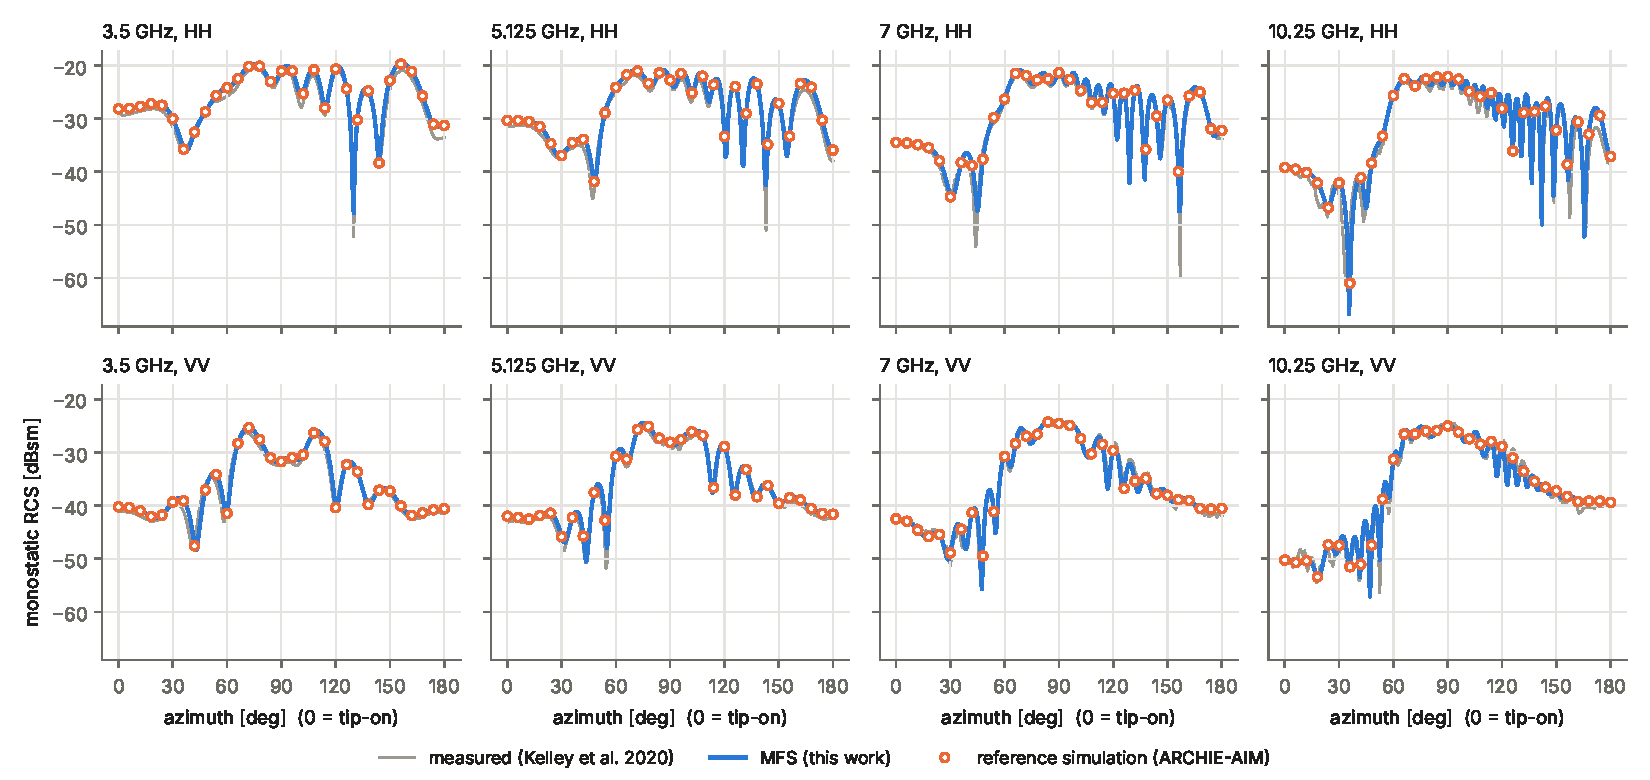
\includegraphics[width=\textwidth]{fig_almond_benchmark.pdf}
  \caption{NASA almond: monostatic radar cross-section against azimuth ($0^\circ$ is nose-on) at four frequencies, HH and VV. MFS, reference simulation and measurements of the Austin benchmark \cite{kelley2020}.}
  \label{fig:almondbench}
\end{figure}

The largest pointwise differences from the reference simulation occur in deep nulls of the HH cross-section. The largest is $4.3$\,dB at $10.25$\,GHz and $35.5^\circ$, in a null at $-66.7$\,dBsm. The MFS is converged there: the layouts $6{:}3$ and $8{:}5$ differ by $0.0006$\,dB on average and by $0.024$\,dB in this null.
The difference is one of position, not of depth. On a grid of $0.02^\circ$ the MFS places this null at $35.66^\circ$ with a depth of $-69.7$\,dBsm, and the cross-section rises by $8$ to $12$\,dB within half a degree on either side. The reference data are sampled every $0.5^\circ$. Shifting the MFS curve by $0.1^\circ$ halves its distance from the reference samples around the null. A shift of this size corresponds to a change of $0.05\%$ in the size of the almond or in the frequency. We conclude that the two simulations agree on this null to within a tenth of a degree, and that the $4.3$\,dB is the price of sampling a sharp null.

At $1.19$, $7$ and $9.92$\,GHz we also compared with Bempp on meshes with $9558$ and $13632$ unknowns. The root-mean-square differences are $0.02$, $0.04$ and $0.12$\,dB for HH and $0.03$, $0.03$ and $0.09$\,dB for VV. At $1.19$\,GHz the MFS cross-section changes by $0.001$\,dB when the row spacing is reduced from $0.5$ to $0.4$.

\section{Discussion and limits}
\label{sec:discussion}

\emph{What the four shapes show together.} The rule that the sources must enclose the singularities of the continued field organises all four layouts. For the sphere any inner sphere will do. For the torus the inner torus must be large enough to enclose the focal ring. For the almond the singular curve is so close to the rim that the sources have to lie on the mid-plane and cluster towards it. For the cube the singular set reaches the surface along every edge, and the sources cluster towards the edges on the skeleton. The singular set touches the surface at the edges and vertices of the cube and at the tip of the almond. There clustering alone converges slowly, and the tail with the exponents of the local expansion restores the accuracy with a few unknowns.

\emph{Where the MFS is ahead of the boundary element code, and where it is not.} On the sphere, the torus and the almond the MFS reaches errors between $10^{-4}$ and $10^{-13}$ in a few seconds, which the low-order boundary element method does not approach (Tables~\ref{tab:sphere}, \ref{tab:torus} and \ref{tab:almond}). On the cube the two methods are close when both use the mirror symmetry of the body. The boundary element method on graded meshes is faster down to an error of $5\times10^{-4}$, by a factor of two at $10^{-3}$. The MFS is faster below $4\times10^{-4}$, by a factor of $1.3$ there and of $2.5$ at $2\times10^{-4}$. The boundary element method flattens near $10^{-4}$, and the MFS continues to $1.5\times10^{-5}$ (\autoref{sec:cubecost}). For a general incident wave the boundary element method is faster down to $4\times10^{-4}$ and the two are level below (\autoref{sec:cubeoblique}). For a cube of two wavelengths the boundary element method is faster down to $10^{-3}$, and the MFS is faster below, by a factor of two at $5\times10^{-4}$ and by more at smaller errors (\autoref{sec:cubek}). In unknowns the MFS is not more economical than the graded boundary element mesh in this range. What it offers on the cube is the rate of convergence.

\emph{Symmetry.} The MFS timings for the torus, the almond and the cube use the symmetry of the body. The symmetry is a property of the body and not of the incident wave, so the timings hold for any wave. For the cube we gave the boundary element method the same symmetry and report both times. For the torus and the almond the Bempp timings do not use it. There it would reduce the time of the boundary element method by a factor of up to four for the almond and more for the torus. It would not reduce its error, which is where the two methods differ on these shapes. Without symmetry our dense least-squares solve would cost far more: the factorisation of one cube matrix with all eight classes together would take $64$ times as long as the eight separate factorisations.

\emph{The boundary element code.} Bempp is a low-order code, and we ran it with dense matrices. We chose its fastest assembly backend, graded the meshes of the cube and raised the quadrature orders where that helped (\ref{sec:bempp}). We did not compare with a high-order or a compressed boundary element method. On the smooth bodies a high-order method would narrow the gap considerably.

\emph{Size.} All bodies are at most nine wavelengths long. The cost of the dense factorisation grows with the cube of the number of unknowns, and we make no claim for larger problems. For the cube we have results at one, two and three wavelengths. At three wavelengths the base grid and its depth must follow the wavelength as well. The layout then converges, and the boundary element solution confirms the field to $7\times10^{-4}$. We have not tuned this case, and in this state the MFS is not faster. With one depth per octave it needs $32$\,s for an error of $8.6\times10^{-4}$. The boundary element method with symmetry, on meshes graded with $g = 1.5$, needs $23$\,s for $1.0\times10^{-3}$ and $56$\,s for $6.9\times10^{-4}$.
%% TODO (authors): the three-wavelength runs are in NOTES.md item 57 (cube_wavenumber.py 3); decide whether they deserve a table.

\emph{Generality.} Each layout was built by hand from the skeleton of its shape. We have no automatic construction for a general body. \autoref{thm:skeleton} covers convex polyhedra only.

\emph{Accuracy on the cube.} The independent boundary element reference confirms the field to $1.0\times10^{-4}$. Below that level the evidence is the convergence of the MFS itself. The last two levels differ by $1.5\times10^{-5}$, from which we estimate an error of $10^{-5}$ for the finest run. The layout with one depth per octave stalls near $1.5\times10^{-4}$.

\emph{The torus.} The bound \eqref{eq:torusradius} is supported by an image argument and by two numerical tests, and it is not proved.

\emph{Nulls of the almond.} In one deep null the MFS and the published reference simulation differ by $4.3$\,dB at the sampled angle. This corresponds to a difference of $0.1^\circ$ in the position of the null (\autoref{sec:almond}). Which of the two positions is correct, we cannot say without a third computation.

\section{Conclusion}

In our examples the method of fundamental solutions converges for Maxwell scattering by bodies with edges and tips when three conditions are met. The sources lie on the skeleton of the body, they cluster towards the singular set, and they are continued below their cut-off by tails with the exponents of the local field. For a convex polyhedron the skeleton is the exact support of the equivalent currents. On the cube successive refinements differ by $1.5\times10^{-5}$ at the finest level, and a graded boundary element computation confirms the field to $1.0\times10^{-4}$. On the NASA almond it reproduces a published reference cross-section to within $0.14$\,dB on average up to $10.25$\,GHz. An automatic construction of the layouts for general shapes is open.


\section*{Code and data availability}
All solvers, the scripts that produce every table and figure, and the stored reference fields are available at \url{https://github.com/sap6/MFS} (folder \texttt{validation}). The measured and simulated almond data are those of the Austin RCS Benchmark Suite \cite{kelley2020}.

%% TODO (authors): acknowledgements; declaration on the use of AI tools as
%% required by the journal (see NOTES.md, section 6).

\appendix
\section{Exponents of the edge tail}
\label{app:edge}

We derive the exponents in \autoref{tab:edgeexp}. Consider one edge of the cube, with coordinates $s$ along the edge and polar coordinates $(\rho,\phi)$ around it. The exterior is the wedge $0<\phi<3\pi/2$. Near the edge the field is a sum of terms of two types \cite{meixner1972},
\begin{align}
  E_s &= a_n(s)\,\rho^{2n/3}\sin(2n\phi/3), & n &= 1,2,\dots, \label{eq:tm}\\
  H_s &= b_n(s)\,\rho^{2n/3}\cos(2n\phi/3), & n &= 0,1,2,\dots, \label{eq:te}
\end{align}
each multiplied by a power series in $\rho^2$. The transverse components follow from $E_s$ and $H_s$ and are one power of $\rho$ lower.

The reflection of \autoref{thm:skeleton} continues each term into the body by the same formula. The two continuations, through the two faces, meet on the bisector half-plane, which is the wall of the skeleton at this edge. With the angle $\psi = \phi - 3\pi/4$ measured from the exterior bisector, the wall is $\psi = \pi$ seen from one side and $\psi = -\pi$ from the other. The angular factors in \eqref{eq:tm} and \eqref{eq:te} are sines and cosines of $2n\psi/3$. Their jump across the wall is proportional to $\sin(2n\pi/3)$ for the part that is odd in $\psi$ and vanishes for the even part. Terms with $n$ a multiple of three do not jump. They are polynomial fields and need no sources.

Let $m$ be the mirror in the bisector plane. A term is even under $m$ if $E_s$ is even in $\psi$ or $H_s$ is odd in $\psi$. For an even term the tangential electric field is continuous across the wall and the tangential magnetic field jumps, so by \eqref{eq:jumps} it leaves only an electric current. An odd term leaves only a magnetic current. Surface currents are tangential, so neither has a component normal to the wall. Reading off the leading jumps gives the densities
\begin{align*}
  J_s &= [H_\rho] \sim \rho^{-1/3}, & J_\rho &= [H_s] \sim \rho^{2/3}, &
  K_s &= [E_\rho] \sim \rho^{1/3},  & K_\rho &= [E_s] \sim \rho^{4/3},
\end{align*}
where $\rho$ is now the depth on the wall. The next terms have exponents larger by two for the electric and by $4/3$ for the magnetic currents.

The tail replaces the current sheet below the deepest free depth $d_J$ by lines at the depths $d_J2^{-i}$. A line stands for the strip of the sheet around it, whose width is proportional to its depth. A density $\rho^{e-1}$ therefore gives the line weights $2^{-ie}$, with $e = 2/3$, $5/3$, $4/3$ and $7/3$ for the four components above.

We checked the exponents numerically at $J = 5$ and $J = 7$. Adding the next term of each expansion changes the error by less than $1\%$ of its value. Lowering the exponents of the two transverse components by one gives an error of $65\%$.

\section{Exponents at a conical point}
\label{app:cone}

Near the vertex of a perfectly conducting cone the field is a sum of terms of two types \cite{vanbladel1996,desmedt1986},
\begin{equation}
  \bE = \nabla\bigl(r^{\nu}\,Y(\hat\bx)\bigr), \qquad \bH = \nabla\bigl(r^{\tau}\,Z(\hat\bx)\bigr),
\end{equation}
where $Y$ and $Z$ are eigenfunctions of the Laplace--Beltrami operator on the part of the unit sphere outside the cone, with Dirichlet and Neumann conditions and eigenvalues $\nu(\nu+1)$ and $\tau(\tau+1)$. The electric type gives $\bE\sim r^{\nu-1}$. The magnetic type gives $\bH\sim r^{\tau-1}$ and $\bE\sim r^{\tau}$.

We compute the eigenvalues by the method of particular solutions in its stable form \cite{betcke2005}. For a trial value of $\nu$ the functions $P_\nu(-\hat\bx\cdot\mathbf{s}_j)$, with $P_\nu$ the Legendre function and $\mathbf{s}_j$ a point of the sphere inside the cone, satisfy the eigenvalue equation on the sphere away from $\mathbf{s}_j$. They are the fundamental solutions of the sphere. The value $\nu$ is an exponent when a combination of them vanishes on the boundary curve without vanishing in the domain. For the almond tip the poles $\mathbf{s}_j$ lie on the focal segment of the elliptic cross-section and cluster towards its ends. For the cube corner they lie inside the spherical triangle that the cube cuts out and cluster exponentially towards its three corners. For a circular cone, where the exponent is known as a root of a Legendre function, the method reproduces it to eight digits. For the almond tip the values are unchanged in five digits when the number of poles is varied from 12 to 36.

\emph{Almond tip.} The tip is an elliptic cone with half-angles $34.09^\circ$ and $12.71^\circ$. \autoref{tab:coneexp} lists the exponents by the parities of the potential under the two mirrors of the almond. Only one exponent is below one, $\nu = 0.29959$, and it belongs to the class that is even under both mirrors. Circular cones with the two half-angles would give $0.377$ and $0.222$.

\emph{Cube vertex.} For the exterior of a corner of the cube we obtain $\nu = 0.45417$, $1.23087$ and $\tau = 0.840$, $1.20635$. The first value agrees with the known exponent of the cube corner \cite{fichera1975}.
%% TODO: compare both tables with De Smedt and Van Bladel 1986 once the paper is at hand.

\begin{table}[htbp]
  \centering
  \caption{Exponents of the elliptic cone at the tip of the almond, by the parities of the potential under the mirrors $y\to-y$ and $z\to-z$.}
  \label{tab:coneexp}
  \begin{tabular}{lll}
    \toprule
    Parity $(y,z)$ & $\nu$ (electric type) & $\tau$ (magnetic type) \\
    \midrule
    even, even & $\mathbf{0.29959}$, $1.46427$ & $1.05604$, $1.98580$ \\
    odd, even  & $1.10372$, $2.24730$ & $0.96803$, $1.96545$ \\
    even, odd  & $1.04120$, $2.10576$ & $0.87905$, $1.75454$ \\
    odd, odd   & $2.01295$, $3.04849$ & $1.97538$, $2.90094$ \\
    \bottomrule
  \end{tabular}
\end{table}

\emph{From exponents to weights.} The tail sources lie on rows that run into the conical point with spacing proportional to the distance $r$. Dipoles of strength $r^{e}$ on such a row produce a field that scales like $r^{e-3}$. A field $r^{\nu-1}$ therefore needs electric dipoles with $e = \nu+2$, and the magnetic type needs magnetic dipoles with $e = \tau+2$.

\section{The singular set of the torus}
\label{app:torus}

We give two arguments for the bound \eqref{eq:torusradius}. Neither is a proof for Maxwell's equations.

\emph{Images.} A plane through the axis cuts the tube in two discs of radius $a$ whose centres are $2R$ apart. For one disc, the singularity at the centre of the other is an exterior source. Its image in the first disc lies at the distance $a^2/(2R)$ from the centre, on the side of the axis. The image of this image lies at $a^2/(2R - a^2/(2R))$, and so on. The sequence $\delta\mapsto a^2/(2R-\delta)$ increases to its fixed point $\delta = R - \sqrt{R^2-a^2}$. The singularities therefore accumulate at the focal ring.

\emph{Static limit.} For Laplace's equation the exterior field of the torus is a series of toroidal harmonics, each of which is singular only on the focal ring. For boundary data from an entire function the series converges outside a smaller torus whose meridian circle has the diameter $[R - a^2/R,\,R]$ and contains both the focal ring and the centre circle.

The general theory of continuation for axially symmetric problems is due to Millar \cite{millar1983}.
%% TODO: read Millar 1983 before submission; if the focal ring is covered there,
%% cite it for (9) and present our tests as a confirmation.

\section{Evaluation of the line sources}
\label{app:lines}

A line source at depth $d$ carries the density \eqref{eq:modes}, and each matrix entry is the integral of a dipole field against one mode. The integrand varies on the scale of the distance between the target and the line, which ranges from $d/3$ to the size of the cube. We organise the quadrature so that most of the work is shared between the targets.

The interval $-1\le u\le1$ is divided into a binary tree of panels. Each panel carries a fixed set of nodes. On the four coarsest levels a panel is wide compared with the scale on which the modes and the map $t(u)$ vary. There we use $12$ Gauss nodes in the physical variable $t$ and replace the kernel by its polynomial interpolant, so that the weights are the exact moments of the Lagrange polynomials against the modes. On the finer levels we use $8$ Gauss nodes in $u$. All nodes and weights are computed once for each depth. A target descends the tree and accepts a panel as soon as the length of the panel is smaller than its distance from the target. A distant target then needs $12$ kernel values for the whole line, and a target at distance $d$ needs a few hundred. The electric and the magnetic line at the same position share the kernel values. The lines of a tail share the nodes, and their kernel values are summed with the tail weights before the modes are accumulated. The eight mirror images of a target are processed together, and their signed sums are written to the matrices of the parity classes in one pass.

The entries agree with those of an adaptive rule with $20$ nodes per panel to a relative accuracy of $10^{-6}$. With $20$ and $10$ nodes in place of $12$ and $8$ the fields of \autoref{tab:cube} change by less than $10^{-6}$, and by less than $10^{-7}$ up to $J = 10$. These node numbers are for a side of one wavelength. They must grow with the wavenumber, because the phase of the kernel varies along a panel in proportion to $k$. At two wavelengths we use $20$ and $10$ nodes, which changes the fields by less than $10^{-10}$ against $32$ and $14$. With $12$ and $8$ the fields there are wrong by up to $2\times10^{-4}$. The norm of the scaled coefficient vector is of order one for all runs in \autoref{tab:cube}, so the quadrature error does not limit the results.

\section{Boundary element settings}
\label{sec:bempp}

We used Bempp-cl version 0.4.2. The electric field integral equation is discretised with Rao--Wilton--Glisson functions as trial functions and scaled N\'ed\'elec functions as test functions. The dense matrix is assembled in double precision, and the system is solved by LU factorisation with LAPACK.

Bempp-cl has two assembly backends. We ran the OpenCL backend on the processor through the PoCL driver. It assembled the matrices of this paper about twenty times faster than the Numba backend, with identical results. For a sphere with $4824$ unknowns the assembly took $4.3$\,s against $96$\,s. All timings use the OpenCL backend. Single precision changed neither the error nor, by more than $20\%$, the time.

The quadrature orders of the library are $4$ for regular and $6$ for singular integrals by default. On meshes graded towards the edges of the cube these orders limit the accuracy at about $10^{-3}$, and we report results with the orders $6$ and $8$ as well as $8$ and $10$. On quasi-uniform meshes the orders made no difference.

The graded meshes of the cube use a tensor grid on each face with the nodes $\pm\tfrac12\bigl(1-(1-|\xi|)^{g}\bigr)$, $\xi$ equally spaced in $[-1,1]$, and each rectangle is cut into two triangles. Of the grading exponents $1$, $1.5$, $2$, $2.5$ and $3$, $g = 2$ gave the smallest errors on the finer meshes with the higher quadrature orders, at one and at two wavelengths. On the coarser meshes with the default quadrature the milder gradings $g = 1.5$ and $1.75$ are better, and at three wavelengths $g = 1.5$ is better throughout. The tables use $g = 2$, and the text quotes the results for the milder gradings where they are faster.

\emph{Mirror symmetry.} For the cube we also solved the boundary element system with the three mirror planes. The graded mesh is built so that it is invariant under the eight reflections. A reflection then acts on the Rao--Wilton--Glisson coefficients as a signed permutation. A current of a given parity class is a combination of symmetrised basis functions, one for each orbit of basis functions under the reflections. The Galerkin equations then need to be tested with only one test function per orbit. We therefore assemble only the rows of the matrix that belong to the test functions of one octant, which Bempp allows by restricting the test space to a part of the mesh. The rows are folded with the symmetrised basis, and each class is solved by an LU factorisation of an eighth of the size. The solution differs from that of the full system by $3\times10^{-5}$ with the default quadrature and by $2\times10^{-6}$ with the orders $8$ and $10$. The quadrature rules of the library are not invariant under the reflections.

We did not use matrix compression, higher-order elements or a second boundary element code. Without the symmetry, at the sizes used here, dense assembly takes between $40\%$ and $90\%$ of the total time and the factorisation the rest. The OpenCL driver limits a single matrix to $4$\,GB on our machine, which is $16384$ unknowns in double precision without the symmetry.


\bibliographystyle{elsarticle-num}
\bibliography{../refs}

\end{document}
